\chapter{Honeynets}
Honeynets bestehen aus mehreren virtuellen oder physikalischen High-Interactive Honeypots, die ein komplettes Netzwerk darstellen\cite{grimes.2003a}\cite{spitzner.2002a}. Jede Netzwerkkomponente und jeder Server kann dabei als Honeypot angesehen werden. Es entsteht somit die Möglichkeit, ein komplettes Produktivnetz nachzustellen, welches dem Hacker den Eindruck vermittelt, in ein produktiv verwendetes Firmennetz eingedrungen zu sein\cite{grimes.2003a}.

\section{Anforderungen eines Honeynets}
\noindent Um ein effektives Honeynet zu erstellen, müssen verschiedenen Anforderungen erfüllt werden. Diese Anforderungen können Honeynets grob ich drei Kategorien unterteilt werden\cite{spitzner.2002a}:\\

\noindent\textbf{Data Control: }\\
Datenkontrolle bedeutet, dass der Betreiber eines Honeypots oder Honeynets die Kontrolle der ein- und ausgehenden Datenpakete behält. Gelingt es dem Hacker dem Honeynetbetreiber diese Kontrolle zu entreißen, besteht die Möglichkeit, dass der Hacker einen Angriff auf das Produktivnetz oder über das Internet startet. Da es sich bei der Datenkontrolle um ein großes Sicherheitsrisiko handelt sollte versucht werden folgende Punkte einzuhalten\cite{spitzner.2002a}:
\begin{itemize}
\item Datenkontrolle sollte automatisiert, jedoch auch manuell stattfinden
\item Die Datenkontrolle sollte mindestens durch zwei Schichten kontrolliert werden (falls eine Anwendung nicht erfolgreich sein sollte)
\item Alle ein- und ausgehenden Verbindungen sollten kontrollierbar bleiben
\item Jede unautorisierte Aktion soll kontrollierbar sein, ein anderes System im Produktivnetz darf nicht angreifbar sein
\item Die Datenkontrolle muss jederzeit durch den Administrator konfigurierbar sein
\item Verbindungen sollen für den Angreifer so schwer wie möglich erkannt werden
\item Mindestens zwei Benachrichtungsmöglichkeiten bei Aktivitäten im Honeynet
\item Auf die Datenkontrolle muss über einen Remote-Zugriff zugegriffen werden können
\end{itemize}
\noindent Die Datenkontrolle muss für den Angreifer unsichtbar sein. Zu strenge Sicherheitsvorkehrungen können den Hacker jedoch verunsichern und ihn auf den Honeypot aufmerksam machen (z.B. ausgehende Verbindungen blockieren). Jedoch kann z.B. eine Limitierung der ausgehenden Verbindungen ein gutes Mittel gegen den Verlust den Datenkontrolle sein\cite{WebHnet.2006b}\cite{spitzner.2002a}. \\

\noindent\textbf{Data Capture: }\\
\noindent Die Informationen, die ein Hacker während eines Angriffes hinterlässt, müssen möglichst reichhaltig und unauffällig dokumentiert werden. Für die Datensammlung gibt es verschiedene Möglichkeiten die Aktionen eine Hackers aufzuzeichnen\cite{grimes.2003a}.
\begin{itemize}
\item Packet Sniffing: Zum aufzeichnen des kompletten Netzverkehrs (ein- und ausgehende Pakete).
\item Keystroke Logging: Das aufzeichnen der vom Hacker ausgeführten Tastenanschläge.
\item Snapshot Software: Vergleicht Betriebssystemkonfigurationen vor- und nach der Kompromittierung und hält die Änderungen fest.
\item Log-Dateien wie z.B. Log-Daten eines Netzwerkgerätes wie Switch und Router
\end{itemize} 
Wichtig bei diesen Programmen ist es, dass sie für den Hacker nicht ersichtlich sein dürfen. Findet der Angreifer eines dieser Programme ist dieser alarmiert und wird die Flucht ergreifen\cite{spitzner.2002a}.
Das Honeynet-Project definiert eine effektive Datenanalyse wie folgt:\cite{spitzner.2002a}
\begin{itemize}
\item Keine aufgezeichneten Honeypot-Daten dürfen lokal auf diesen gespeichert werden (diese könnten vom Angreifer erkannt und modifiziert werden). Als Honeypot-Daten zählen alle Daten die bezüglich des Honeypots und dessen Umgebung aufgezeichnet werden.
\item Folgende Aktivitäten müssen ein Jahr lang aufgezeichnet werden: Netzwerkaktivitäten, Systemaktivitäten, Anwendungsaktivitäten und Benutzeraktivitäten.
\item Der Honeypot oder Honeynet Administrator muss jederzeit ortsunabhängig auf aufgezeichnete Daten Zugreifen können.
\item Aufgezeichnete Daten müssen für zukünftige Analysen automatisch archiviert werden.
\item Für jeden aktive Honeypot muss eine standardisierte Log-Datei existieren.
\item Für jeden kompromittierten Honeypot muss ein standardisierte Log-Datei existieren.
\item Alle gesammelten Daten müssen die GMT Zeitzone verwenden. Daten können zwar mit der lokalen Zeitzone aufgezeichnet werden, müssen jedoch für eine Analyse in das GMT Zeitformat konvertiert werden.
\item Anwendungen, die zur Aufzeichnung von Aktivitäten dienen, müssen sicher gegen Modifikationen sein, um die Integrität der aufgezeichneten Daten sicherzustellen.
\end{itemize}

\noindent\textbf{Data Collection: }\\
\noindent Bei einem verteilten System wie z.B. bei einem Honeynet muss es eine zentrale Stelle geben, in der die Informationen gesammelt und gespeichert werden. Daten werden nie direkt auf einem Honeypot protokolliert, sondern an ein zentrales System übertragen. Wichtig hierbei ist es, dass die Daten sicher und unverändert an das System übertragen werden. Der Angreifer soll nicht die Möglichkeit haben einen Angriff zu vertuschen, oder gar das System selbst anzugreifen\cite{WebHnet.2006b}. Die Anforderungen an die Datensammlung kann in vier Elemente unterteilt werden\cite{spitzner.2002a}:
\begin{itemize}
\item Jeder Honeypot im Honeynet soll in der Sammlung identifizierbar sein. Dies kann z.B. durch eine Art \acf{IP/DNS} gemappte Datenbank erreicht werden.
\item Die Daten müssen vom Honeypot sicher auf das Sammelnde System übertragen werden. Die Integrität der Daten darf nicht während der Übertragung verändert werden können.
\item Eine Möglichkeit zur Anonymisierung der Daten. 
\item Eine Standardisiertes \acf{NTP}, um sicherzustellen dass alle Daten richtig synchronisiert wurden.
\end{itemize}

\noindent\textbf{Data Analysis: }\\
\noindent Die gewonnenen Informationen müssen dem Zweck entsprechend ausgewertet werden. Je nach Ziel des Honeypots müssen z.B. Gegenmaßnahmen getroffen, oder aus dem gelernten Wissen Schlüsse gezogen werden, um in Zukunft eine Kompromittierung eines Produktivsystems zu verhindern\cite{WebHnet.2006b}.

\section{Architektur eines Honeynets}
Es gibt zwei verschieden Arten von Architekturen die sich im Laufe der Zeit durchgesetzt haben. Diese werden in Generation I und Generation II Honeynets (Abk. GenI und GenII) unterteilt.\\
\subsection{GenI Honeynet}
Bei einem GenI Honeynet wird das gesamte Netz durch eine Firewall in drei Teile unterteilt. Der erste Teil ist das Produktivnetz indem sich das zentrale Management System befindet. Der zweite Teil ist das Internet, welcher das Zugangsmedium des Angreifers darstellt. Der dritte und letzte Teil ist das Honeynet\cite{WebGenI.2006b}. 

GenI Honeynets gelten als die ersten richtigen High-Interactive Honeypots, da sie weit mehr Informationen als normale Honeypot, und unbekannte Angriffe aufzeichnen können\cite{spitzner.2002a}.

Der Prozess der Datensammlung beginnt bereits mit passieren der Firewall. Dort können Informationen wie die verwendeten Protokolle, Zeitstempel,IP-Adressen und Ports gesammelt werden. Außerdem wird hier kontrolliert wie oft der Angreifer eine Verbindung eingehen kann (Data Control). Wie viele Versuche zugelassen werden hängt vom Verwendungszweck des Honeynets ab. Der Router zwischen Honeynet und Firewall unterstützt diese auf zwei verschiedene weisen. Zum Einem versteckt er die Firewall vor dem Hacker. Der Angreifer denkt, er greift auf einen produktiven Router zu. Zum Anderen unterstützt er die Firewall in Sachen Zugriffskontrolle. So kann ein Single-Point-of-Failure vermieden werden\cite{grimes.2003a}\cite{WebGenI.2006b}. 

Ein \acf{IDS}-System steht nun noch zwischen dem Angreifer und den Honeypots. Dieses ist meist über einen Switch (oder wie in Abb. \ref{hnet:geni} mit einem Router) mit dem gesamten Honeynet verbunden. Dort werden alle Netzwerkaktivitäten protokolliert und bei bestimmten Angriffsmustern gegebenenfalls ein Alarm ausgelöst\cite{spitzner.2002a}. 

\begin{figure}[ht]
    \centering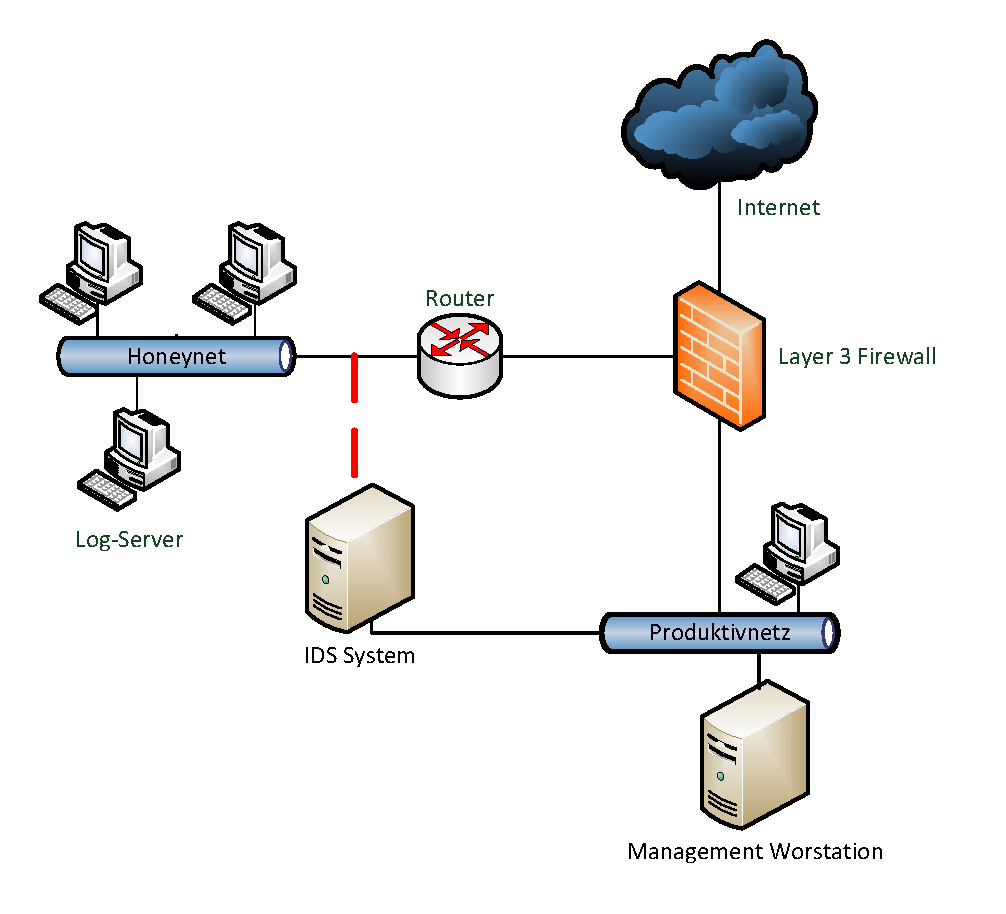
\includegraphics[scale=0.5]{Bilder/GenI.pdf}
  \caption{GenI Honeynet}
  \label{hnet:geni}
\end{figure}

\noindent Die GenI Technologie bietet sich besonders an, um automatisierte oder Anfänger-Hacks zu erkennen. Meist handelt es sich dabei um Ziele, deren Schwachstelle zufällig entdeckt wird, und es dadurch zu einem Angriff kommt. 
Die Architektur ist nicht effektiv für fortgeschrittene Angreifer, oder Hacker, die ein bestimmtes System angreifen wollen. Zum einen sind diese relativ einfach über einen Fingerprint ausfindig zu machen, zum Anderen bestehen sie meist aus einer Standardinstallation eines Betriebssystems, weswegen sie für Angreifer meist uninteressant wirken\cite{spitzner.2002a}.\\

\noindent\textbf{Methoden zur Datenkontrolle}\\
\noindent Die Datenkontrolle eines GenI Honeypots besteht im Grunde aus der Layer 3 Firewall, die das Produktivnetz vom Honeynet trennt. Die Firewall erlaubt jeglichen Zugriff in das Netz, limitiert jedoch die ausgehenden Verbindungen (nicht Pakete). Der Firewall wird vom Administrator eine Grenze für ausgehende Verbindungen mitgeteilt, nach erreichen dieser wird jeder ausgehender Verbindungsversuch geblockt. Je mehr Verbindungen erlaubt sind, desto mehr Freiheiten hat der Hacker seine Aktionen durchzuführen. Um den Schaden zu minimieren die der Hacker verursacht, kann auch eine geringe Grenze gewählt werden. Automatisierte Attacken können so z.B. weiterhin festgestellt werden. Das Honeynet Project empfiehlt hierfür die Linux Firewall IPTables oder als kommerzielle Version FireWall-1 \cite{spitzner.2002a}.\\

\noindent\textbf{Methoden zur Datenaufzeichnung}\\
\noindent Die Datenaufzeichnung eines GenI Honeynets muss, wie zuvor definiert (vgl. Kapitel 3.1), für den Angreifer unsichtbar sein. Die Daten, die gesammelt werden, dürfen nicht lokal auf dem Honeypot gespeichert werden. Um dies zu verwirklichen werden die Daten in verschiedenen Schichten.
Die erste Schicht ist die Logging-Aktivität auf der Firewall. Alle Daten, die in das Honeynet gelange, müssen zunächst durch die Firewall. Dort können zwar keine Informationen wie Tastendrücke oder Packet-Payloads aufgezeichnet werden, jedoch können Protokoll Header, in denen sich Informationen wie Zeitpunkt, Quell- und Zieladresse sowie Quell- und Zielport befinden, ausgelesen und aufgezeichnet werden\cite{spitzner.2002a}. 

Die zweite Schicht ist das IDS-System, welches mit dem Produktivnetz und dem Honeynet jeweils mit einem Interface verbunden ist. Das Interface, dass mit dem Honeynet verbunden ist besitzt keine IP-Adresse. Es gilt als passives Interface (rote Linie in Abb. \ref{hnet:geni}), welches den kompletten Datenverkehr des Honeynets aufzeichnet, jedoch keine Angriffsfläche für den Hacker bietet, da es keine IP-Adresse besitzt. Das zweite Interface erlaubt es dem Administrator im Produktivnetz auf die gesammelten Daten zuzugreifen. Das IDS zeichnet die kompletten Datenpakete mit Payload auf und stellt diese später für eine Datenanalyse zur Verfügung. Die zweite Aufgabe des IDS ist es, eine Warnung bei ungewöhnlichen Aktivitäten zu geben.

Die dritte Schicht stellen die Honeypots selbst dar. Alle System und 
\subsection{GenII und GenIII Honeynets}
Die zweite Generation von Honeynets verwendet ein Gateway, welches die Funktionen der in GenI verwendetet Komponenten enthält, und diese noch weiter ergänzt. Dieses Gateway (meist Honeywall genannt) besteht nicht wie in GenI aus einem Layer-3 Router sondern aus einer Layer-2 Bridge. Dies verhindert z.B. dass der Angreifer über die TTL-Zähler eines IP-Paketes dn Router erkennen würde. Alle zuvor genannten Anforderungen werden in der Honeywall erfüllt. Für die Datenkontrolle werden hier wie in GenI die Verbindungen limitiert (oft mit dem Programm IPTables), um so DOS-Angriffe zu vermeiden und die Kontrolle über die Verbindungen zu erhalten. Zusätzlich bietet sich nun auch die Möglichkeit Zugriffe die über bestimmte Protokolle einzeln zu limitieren.

Ein IDS oder IPS verhindert weiterhin das der Hacker vom Honeynet aus einen Angriff auf das Produktivsystem oder in das Internet starten kann. Die Zugriffskontrolle und das IDS sammeln wie beim GenI Honeypot die Daten. In Abb. \ref{hnet:genii} befindet sich ein Beispiel einer GenII Honeynet Architektur.
\\
\begin{figure}[]
    \centering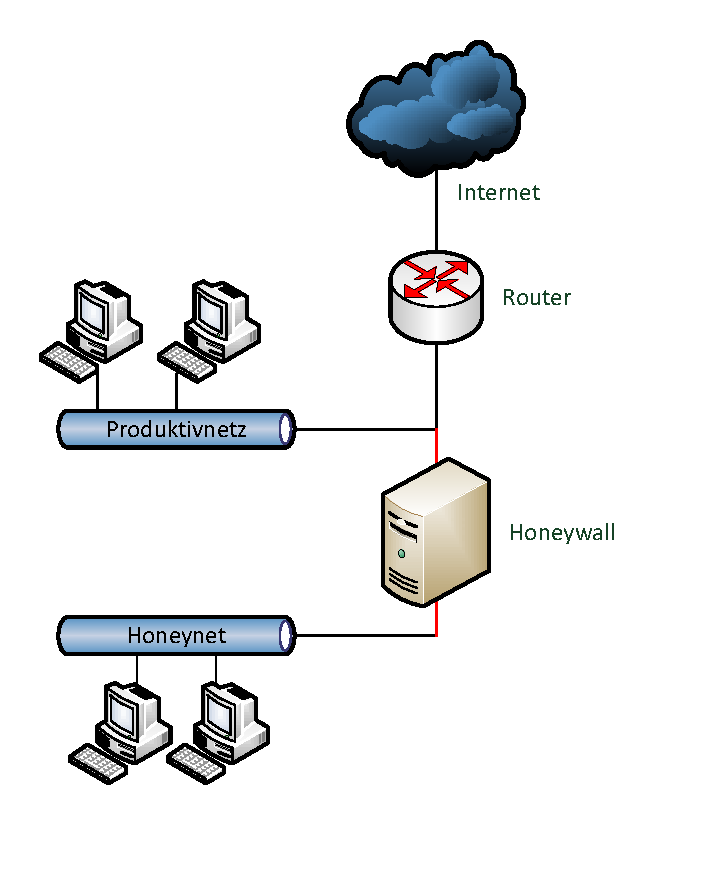
\includegraphics[scale=0.5]{Bilder/GenII.pdf}
  \caption{GenII Honeynet}
  \label{hnet:genii}
\end{figure}
\\
\noindent Ende 2004 wurde die vorerst letzte Generation von Honeynets vorgestellt. Ein GenIII Honeynet besitzt die selbe Netzwerkarchitektur wie dessen Vorgänger, behebt jedoch einig dessen Schwachstellen. Bei dem Versuch einen Honeynet Standard und eine Möglichkeit zu finden, ein Honeynet leichter zu Erstellen, veröffentlichte das Honeynet-Project (www.honeynet-project.org) eine CD, die alle Anforderungen eines Honeynets beinhaltet. Diese CD (\emph{Roo} genannt) wird als dritte Generation angesehen. Die aktuelle Version (1.4, Stand: 2014) bietet neben der verbesserten Datensammlung ,eine grafische Web-Oberfläche zur Datenanalyse, und unterstützt weiter Tools wie Sebek und Hflow2 (Siehe Kapitel Tools).

